\documentclass{article}
\usepackage[a4paper, margin=3mm, landscape]{geometry}
\usepackage{multicol}
\usepackage{xcolor}
\usepackage{enumitem}
\usepackage{amsmath}
\usepackage{amsfonts}
\usepackage{listings}
\usepackage{soul}
\usepackage{graphicx}

\pdfinfo{
    /Title (CS2105.pdf)
    /Creator (TeX)
    /Producer (pdfTeX 1.40.0)
    /Author (Jason Qiu)
    /Subject (CS2105)
    /Keywords (CS2105, nus, cheatsheet, pdf)
}

\graphicspath{ {./img/} }

\pagestyle{empty}
\setcounter{secnumdepth}{0}
\setlength{\columnseprule}{0.25pt}

% Redefine section commands to use less space
\makeatletter
\renewcommand{\section}{\@startsection{section}{1}{0mm}%
    {-1ex plus -.5ex minus -.2ex}%
    {0.5ex plus .2ex}%x
{\normalfont\large\bfseries}}
\renewcommand{\subsection}{\@startsection{subsection}{2}{0mm}%
    {-1explus -.5ex minus -.2ex}%
    {0.5ex plus .2ex}%
{\normalfont\normalsize\bfseries}}
\renewcommand{\subsubsection}{\@startsection{subsubsection}{3}{0mm}%
    {-1ex plus -.5ex minus -.2ex}%
    {1ex plus .2ex}%
{\normalfont\small\bfseries}}%
\makeatother

% Adjust spacing for all itemize/enumerate
\setlength{\leftmargini}{0.5cm}
\setlength{\leftmarginii}{0.5cm}
\setlist[itemize,1]{leftmargin=2mm,labelindent=1mm,labelsep=1mm}
\setlist[itemize,2]{leftmargin=2mm,labelindent=1mm,labelsep=1mm,label=$\bullet$}

% Font
\renewcommand{\familydefault}{\sfdefault}

% Define colors for math formulas
\definecolor{myblue}{cmyk}{1,.72,0,.38}
\everymath\expandafter{\the\everymath \color{myblue}}

% Custom command for keywords
\definecolor{highlight}{RGB}{251,243,218}
\newcommand{\keyword}[2][]{\sethlcolor{highlight}\hl{\textbf{#2}} #1 - }
\newcommand{\ilkeyword}[1]{\sethlcolor{highlight}\hl{\textbf{#1}}}

% Define colors and style for code
\definecolor{codegreen}{rgb}{0,0.6,0}
\definecolor{codegray}{rgb}{0.5,0.5,0.5}
\definecolor{codered}{HTML}{CC241D}
\definecolor{backcolor}{rgb}{0.95,0.95,0.95}
\lstdefinestyle{codestyle}{
    backgroundcolor = \color{backcolor},
    commentstyle = \color{codegray},
    keywordstyle = \color{codered},
    stringstyle = \color{codegreen},
    basicstyle = \ttfamily,
    breakatwhitespace = false,
    showstringspaces = false,
    breaklines = true,
    showtabs = false,
    tabsize = 2
}
\lstset{style = codestyle}

% -----------------------------------------------------------------------
\begin{document}
\begin{multicols*}{3}
\footnotesize

% Title box
\begin{center}
    \fbox{
        \parbox{0.8\linewidth}{
            \centering \textcolor{black}{
                {\Large\textbf{CS2105}} \\
                \normalsize{AY22/23 Sem 2}} \\
                {\footnotesize \textcolor{gray}{github.com/jasonqiu212}}
        }
    }
\end{center}

\section{01. Introduction}

\begin{itemize}
    \item \keyword{Network Edge}{Hosts (Clients and servers)}
    \item \keyword{Access Networks}{Wired and wireless communication links}
    \item \keyword{Network Core}{Network of interconnected routers}
\end{itemize}

\subsection{Network Core}

\subsubsection{Packet-Switching}

\begin{itemize}
    \item Host breaks messages into packets of $L$ bits 
    \item Transmits packets into access network at transmission rate $R$ (aka Link bandwidth, capacity)
\end{itemize}

\[\text{Packet Transmission Delay} = \frac{\text{Packet Size (bits)}}{\text{Transmission Rate (bits/sec)}}\]

\begin{itemize}
    \item \keyword{Store and Forward}{Entire packet must arrive at router before being transmitted to next link}
\end{itemize}

\subsubsection{Key Functions of Network Core}

\begin{itemize}
    \item \keyword{Routing}{Determines source-destination routes taken by packets (How we get the hashtable)}
    \item \keyword{Forwarding}{Move packets from router's input to correct router output}
\end{itemize}

\subsubsection{Circuit Switching}

\begin{itemize}
    \item Resources reserved for call between source and destination
    \item Pros: Betrer performance
    \item Cons: More resources
\end{itemize}

\subsubsection{Internet Structure}
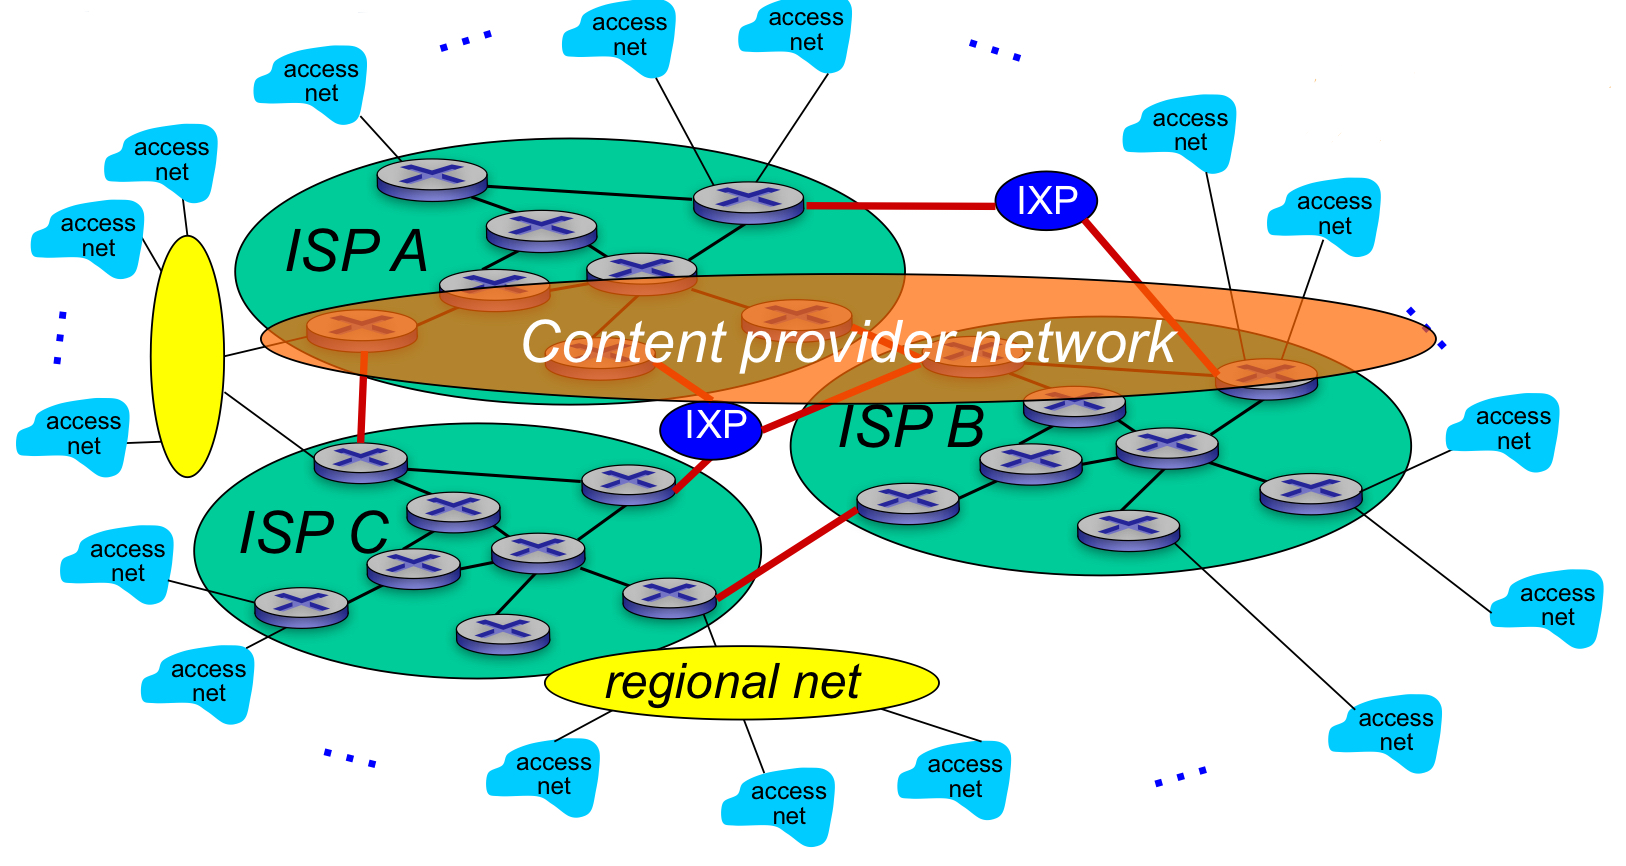
\includegraphics[scale=0.15]{internet}

\begin{itemize}
    \item End systems connect to Internet via \textbf{Access Internet Service Providers (ISPs)}
    \item ISPs connect to larger global ISPs (usually competitors)
    \item Large ISPs connect via \textbf{peering links} or \textbf{internet exchange points (IXP)}
    \item \keyword{IXP}{Physical place with routers from different ISPs}
    \item \keyword{Regional Networks}{Smallers ISPs}
    \item \keyword{Content Provider Networks}{Provide content close to end users}
\end{itemize}

\subsection{Loss, Delay, and Throughput}

\subsubsection{Packet Loss}

\begin{itemize}
    \item If Arrival Rate $>$ Transmission Rate, packets will queue and can be dropped if queue fills up
    \item Solutions: Lost packets can be retransmitted
\end{itemize}

\subsubsection{Packet Delay}

\[d_{\text{nodal}} = d_{\text{proc}} + d_{\text{queue}} + d_{\text{trans}} + d_{\text{prop}}\]

\begin{itemize}
    \item \keyword{Nodal Processing}{($d_{\text{proc}}$) Check for bit errors and determine output link}
    \item \keyword{Queueing Delay}{($d_{\text{queue}}$) Time at queue waiting for transmission}
    \item \keyword{Transmission Delay}{($d_{\text{trans}}$) Time to load packet onto link}
    \begin{itemize}
        \item $d_{\text{trans}} = \frac{L}{R}$ where $L$ is packet length and $R$ is link bandwidth
    \end{itemize}
    \item \keyword{Propagation Delay}{($d_{\text{prop}}$) Time for 1 bit to reach end of link}
    \begin{itemize}
        \item $d_{\text{prop}} = \frac{d}{s}$ where $d$ is length of link and $s$ is propagation speed
    \end{itemize}
\end{itemize}

\subsubsection{Throughput}

\begin{itemize}
    \item Rate at which bits transferred between hosts
    \begin{itemize}
        \item Different from transmission rate (Theoretical upper bound)
    \end{itemize}
    \item Average: Rate over long period of time
    \item Instantaneous: Rate at given point in time
\end{itemize}

\subsection{Protocol Layers and Service Models}

\begin{itemize}
    \item \keyword{Protocol}{Defines format, order of messages sent and received, and actions taken on message transmission}
    \item Networks are complex with many components. How can we organize its structure?
    \item \keyword{Layering}{Each layer implements a service by doing something within layer and relying on services provided by layer below it}
    \begin{itemize}
        \item Explicit structure allows us to make sense of complex components
        \item Easy maintenance (Like OOP, change in 1 layer should not affect others)
    \end{itemize}
\end{itemize}

\subsubsection{Internet Protocol Stack}

\begin{enumerate}
    \item Application
    \item Transport
    \item Network
    \item Link
    \item Physical
\end{enumerate}

\section{02. Application Layer}

\begin{itemize}
    \item Programs that run on end systems, and not on network-core devices
\end{itemize}

\subsection{Client-server Architecture}

\begin{itemize}
    \item Server: Always-on host, Permanent IP address
    \item Clients: Communicates with server, Intermittently connected, Dynamic IP addresses, Do not communicate with each other directly
\end{itemize}

\subsection{P2P Architecture}

\begin{itemize}
    \item Peers request service from other peers and provide service in return
    \item No always-on server, Intermittently connected, Dynamic IP addresses
    \item \keyword{Self Scalability}{New peers offer new services and demands}
\end{itemize}

\subsection{Process}

\begin{itemize}
    \item \keyword{Process}{Program running in host}
    \item \keyword{Inter-process Communication}{How 2 processes in 1 host communicate}
    \item \keyword{Messages}{Processes in different hosts communicate by exchanging this}
    \item \keyword{Client Process}{Process that initiates communication}
    \item \keyword{Server Process}{Process that waits to be contacted}
    \item \keyword{Socker}{Process sends/receives messages to/from its socket (like a door)}
    \begin{itemize}
        \item Outside of socket, transport layer delivers message
    \end{itemize}
\end{itemize}

\subsection{Addressing Processes}

\begin{itemize}
    \item Motivation: IP address is not enough to address process, since many processes can be running on same host
    \begin{itemize}
        \item \keyword{Identifier}{IP address and port number}
        \item \keyword{Port Number:}{Associated with process on host}
    \end{itemize}
\end{itemize}

\subsection{Transport Protocol Services}

\begin{enumerate}
    \item \keyword{TCP}{Transmission Control Protocol}
    \begin{itemize}
        \item Reliable transport
        \item Flow control: Sender does not overwhelm receiver
        \item Congestion control
        \item Connection-oriented: Setup required between client and server
    \end{itemize}
    \item \keyword{UDP}{User Datagram Protocol}
    \begin{itemize}
        \item Unreliable data transfer
        \item Fast
    \end{itemize}
\end{enumerate}

\subsection{App-layer Protocol}

\begin{itemize}
    \item Types of messages exchanged (e.g. Request or response)
    \item Message syntax: How fields are delineated
    \item Messages semantics: Meaning of information in fields
\end{itemize}

\subsection{HTTP}

\begin{itemize}
    \item \keyword{Hypertext Transfer Protocol}{Web's application layer protocol}
    \item Motivation: Web page consists of objects (HTML, images). Need method to request/send web objects.
    \item Follows client/server model
    \item Uses TCP
    \item \keyword{Stateless}{Server maintains no information about past requests}
\end{itemize}

\subsubsection{Non-persistent HTTP}

\begin{itemize}
    \item At most 1 object sent over TCP connection
    \item Downloading multiple objects requires multiple TCP connections
\end{itemize}

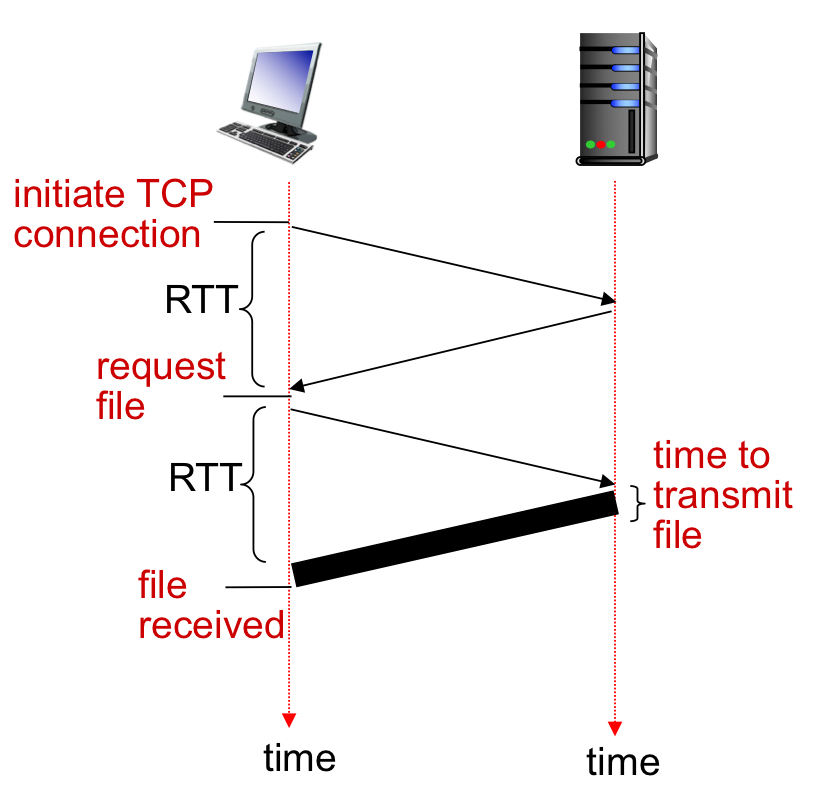
\includegraphics[scale=0.15]{non-persistent-http}

\begin{itemize}
    \item Server closes TCP connection after sending file
    \item \keyword{Return Trip Time}{(RTT) Time for small packet to travel from client to server and back}
    \item Response Time: 2 RTT + File transmission time
\end{itemize}

\subsubsection{Persistent HTTP}

\begin{itemize}
    \item Multiple objects can be sent over single TCP connection
    \item Server leaves TCP connection open after sending response
    \item As little as one RTT for all referenced objects
\end{itemize}

\subsubsection{HTTP Request Message}

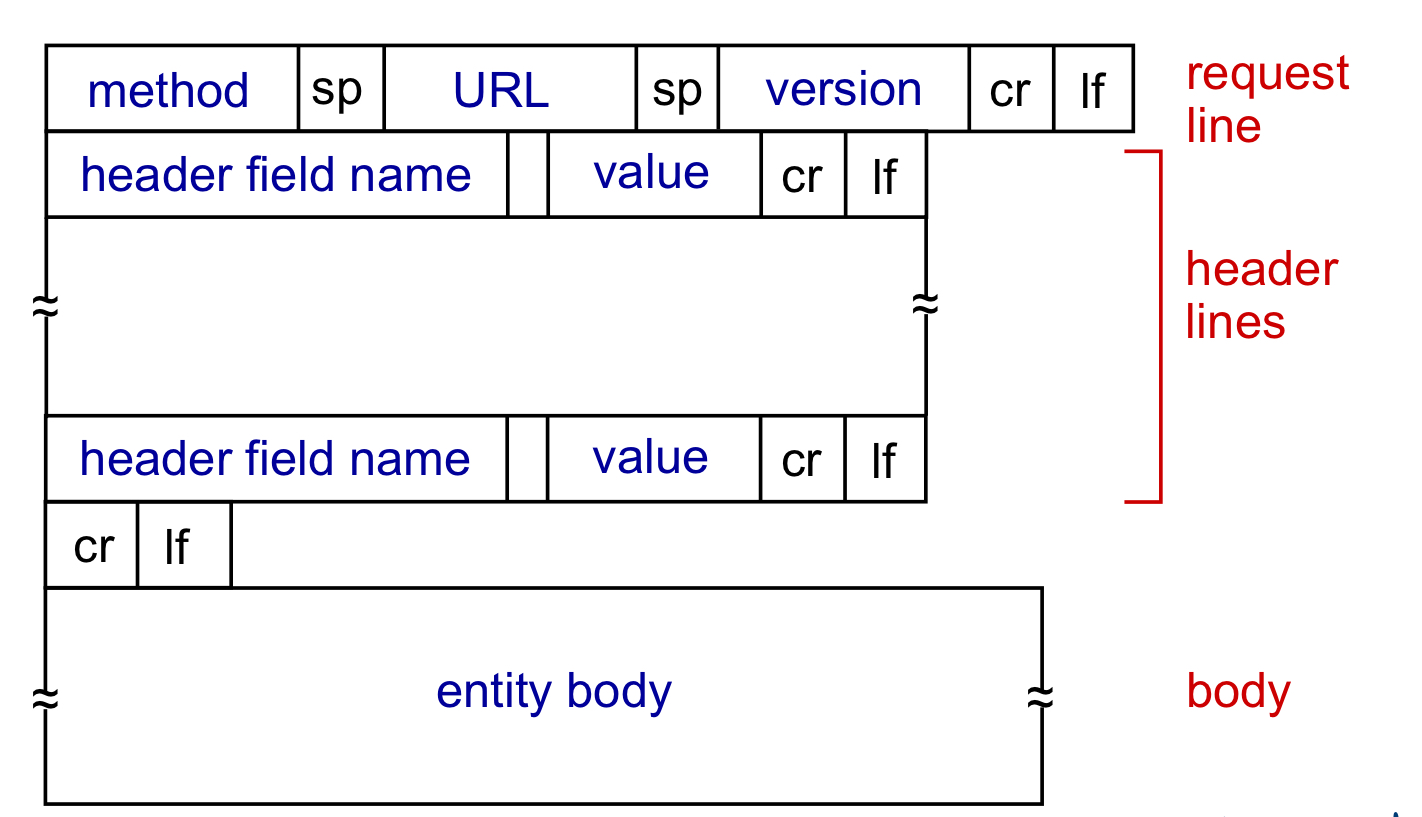
\includegraphics[scale=0.12]{http-request}

\begin{itemize}
    \item To upload form input: \keyword{POST method}{Input uploaded via entity body} and \keyword{URL method}{Input uploaded in URL field of GET method}
    \item \keyword{HTTP/1.0}{GET, POST, HEAD (Ask server to leave request object out of response)}
    \item \keyword{HTTP/1.1}{GET, POST, HEAD, PUT, DELETE}
\end{itemize}

\subsubsection{HTTP Response Message}

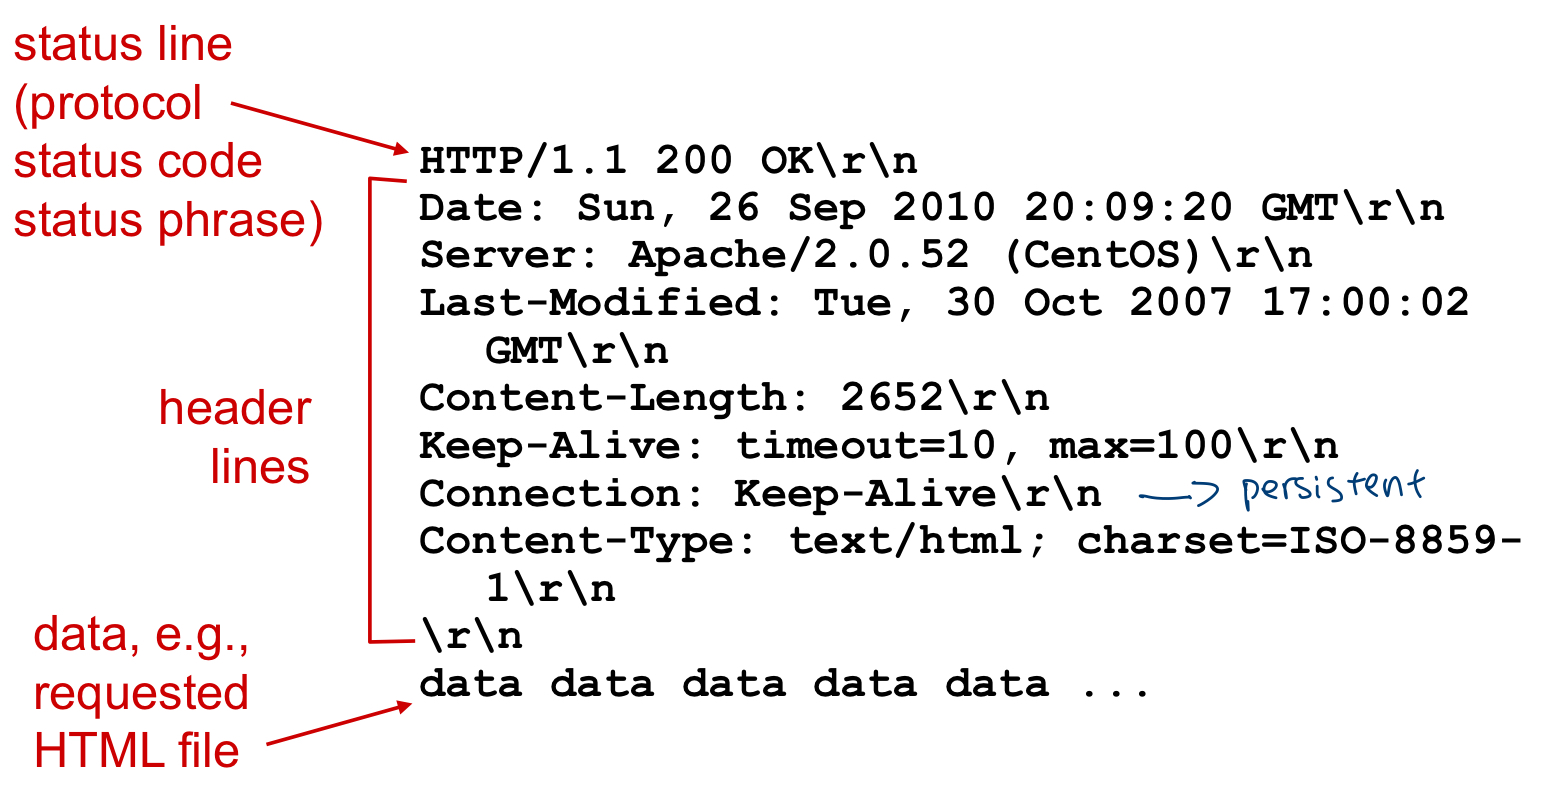
\includegraphics[scale=0.15]{http-response}

\subsubsection{Cookies}

\begin{itemize}
    \item Maintains state on client side
    \item Components: Cookie header for HTTP response, Cookie header for HTTP, request, Cookie file on user's host (Key-value pair), Database on server
\end{itemize}

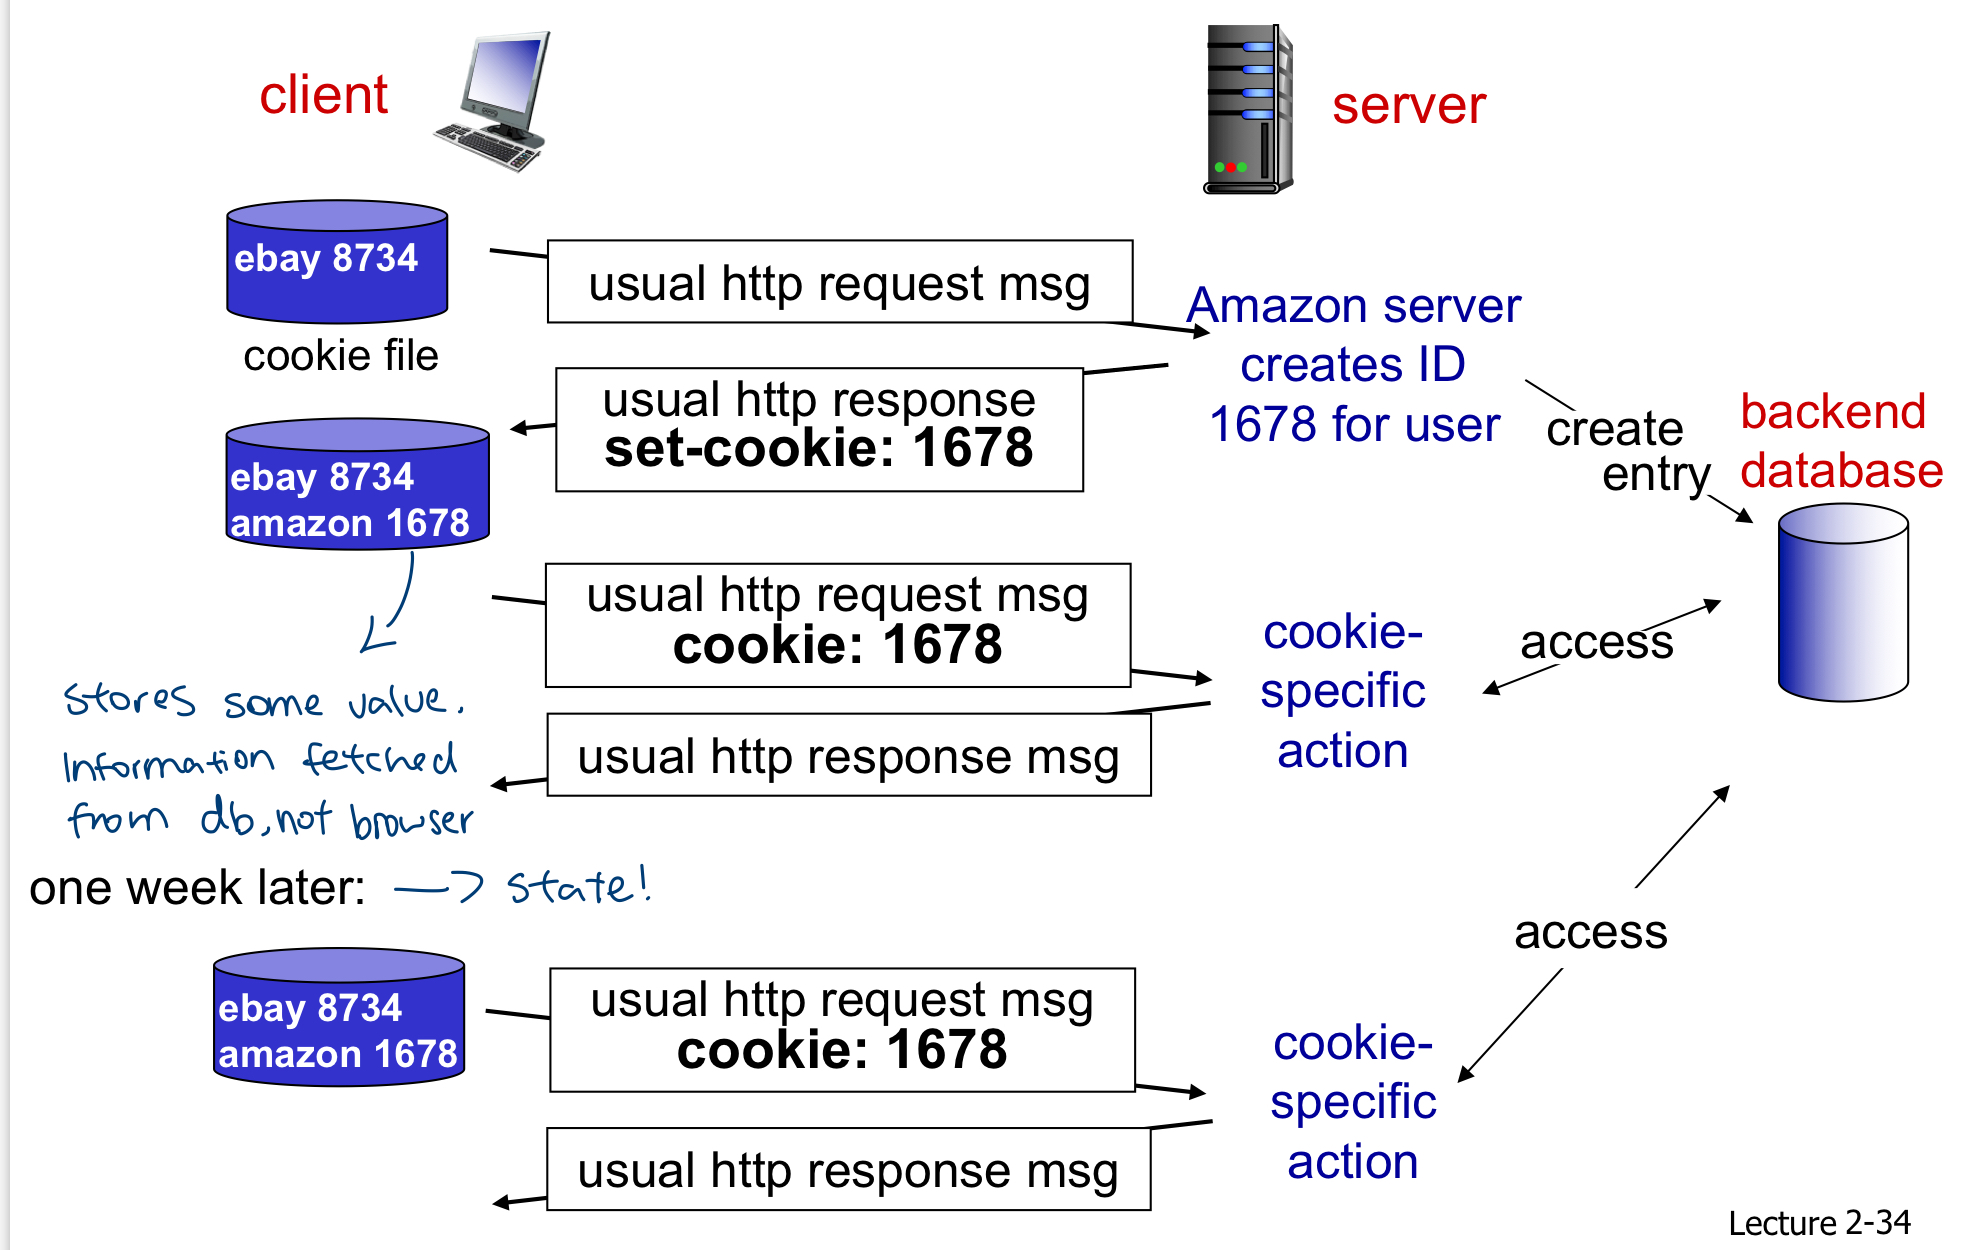
\includegraphics[scale=0.12]{cookies}

\subsubsection{Web Cache (Proxy Server)}

\begin{itemize}
    \item Goal: Fulfill request without involving origin server via caching
    \item Browser sends all HTTP requests to cache
    \item Pros: Faster, Reduces traffic to origin server
    \item Cons: What if origin server updates?
    \begin{itemize}
        \item \keyword{Conditional GET}{Origin server doesn't send object if cache has updated version}
        \item Cache: Specifies date of cached copy in HTTP request to origin
        \item Origin Server: Response contains no object if cached object is updated
    \end{itemize}
\end{itemize}

\subsection{Domain Name System}

\begin{itemize}
    \item Maps between IP address and name (e.g. yahoo.com)
    \item Implemented using distributed and hierarchical databases
    \item Application-layer protocol
    \item \keyword{Local DNS Name Server}{Local cache of name-to-address mapping. Forwards query into hierarchy.}
    \begin{itemize}
        \item \keyword{Time to Live}{(TTL) Cached mappings disappear after some time}
    \end{itemize}
    \item \keyword{Root Name Server}{Contacted by local name server that cannot resolve name. Provides IP address of TLD servers.}
    \item \keyword{Top-level Domain Server}{(TLD) Provides IP address of authoritative server}
    \item \keyword{Authoritative DNS Server}{Organization's own DNS server. Provides mappings for organization's named hosts.}
    \item Iterated query: "Not sure, ask this server"
\end{itemize}

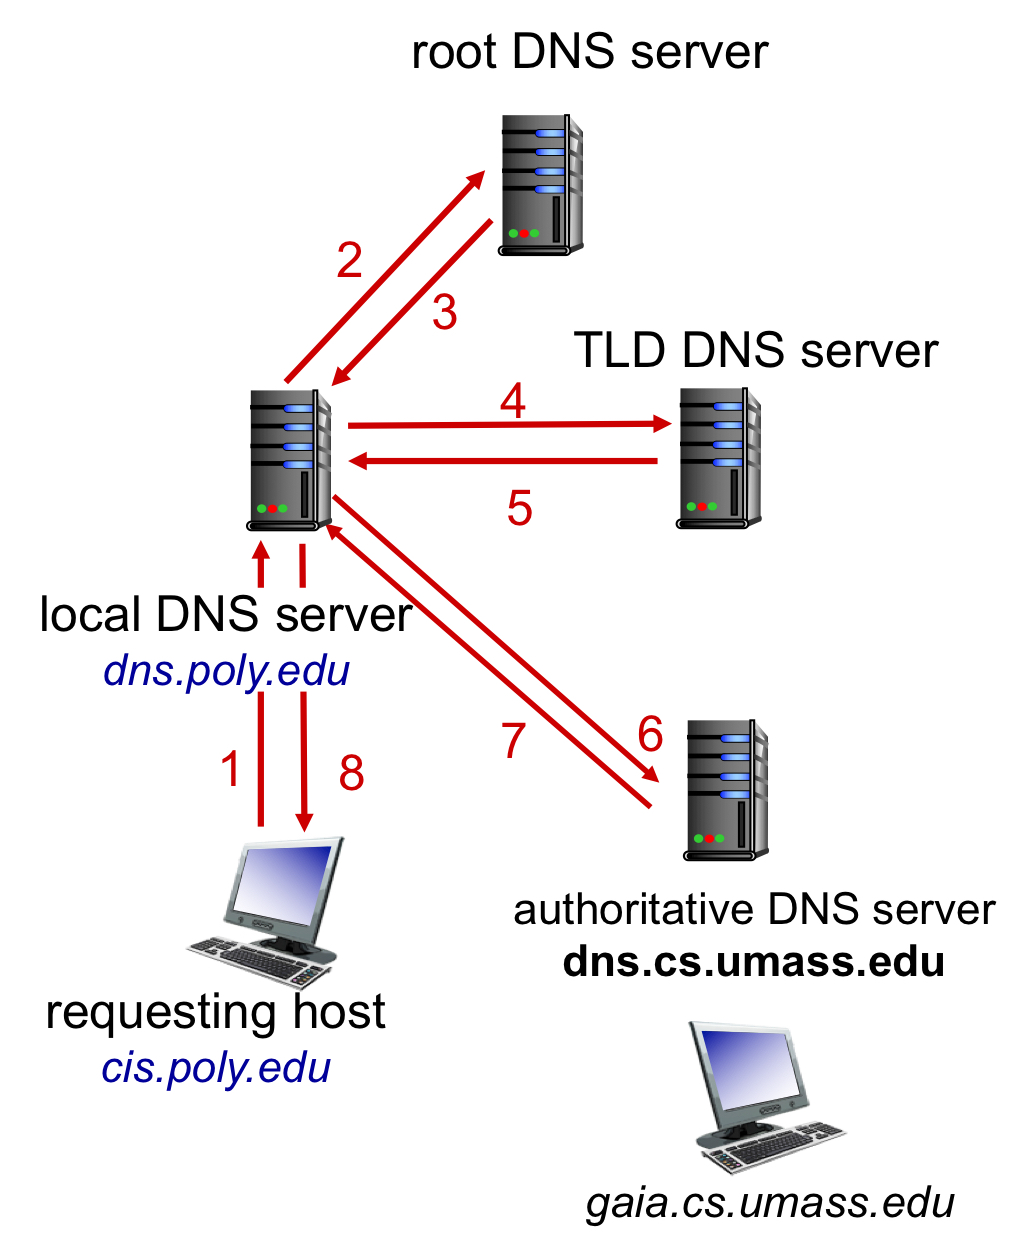
\includegraphics[scale=0.1]{dns-iterative-query}

\begin{itemize}
    \item Recursive query: "Okay, let me find for you"
    \begin{itemize}
        \item Heavy load on upper levels of hierarchy
    \end{itemize}
\end{itemize}

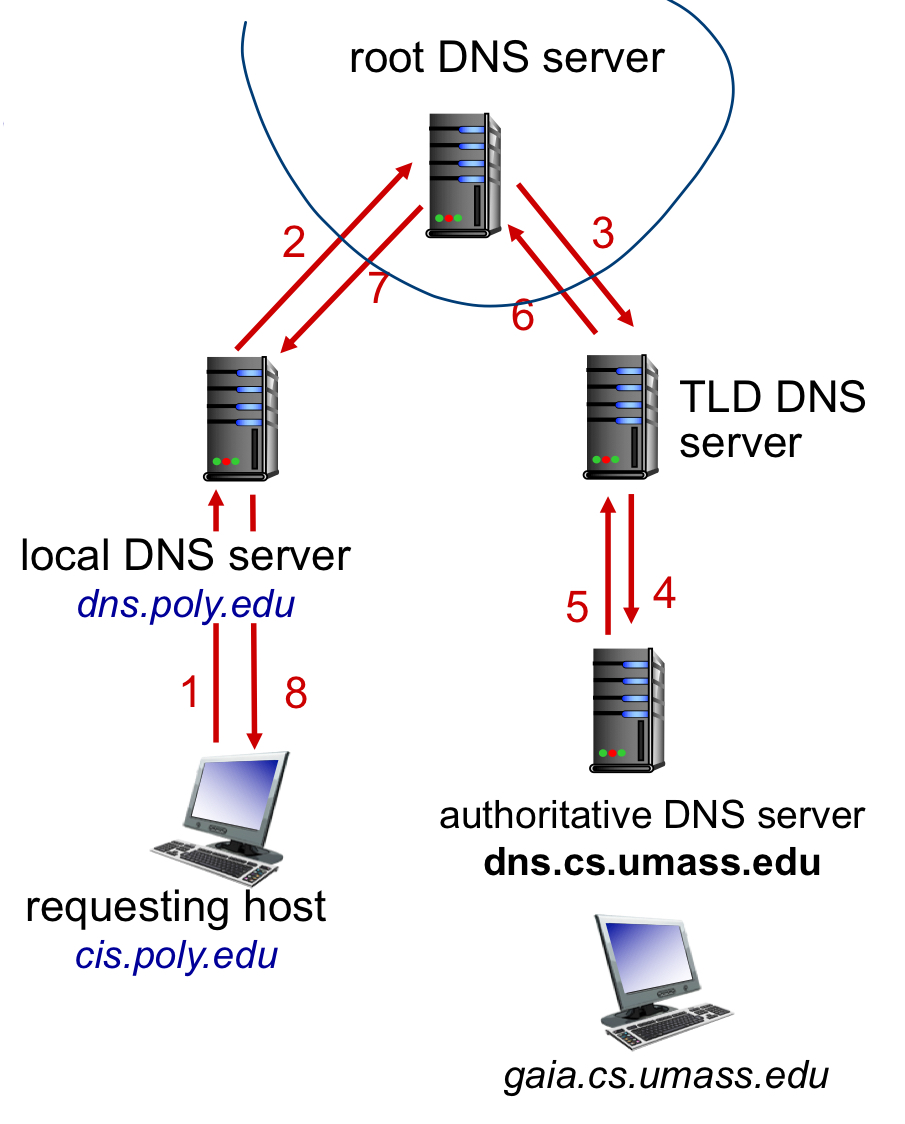
\includegraphics[scale=0.1]{dns-recursive-query}

\end{multicols*}
\end{document}
